\apendice{Especificación de Requisitos}
\section{Diagrama de casos de uso}
En la figura \ref{fig:Diagrama Casos de uso}, se puede observar el diagrama de casos de uso definido para el uso del dispositivo. 

Existen 3 personas diferentes, ingeniero, usuario (sanitario) y el paciente, con funciones diferentes 
\begin{figure}
    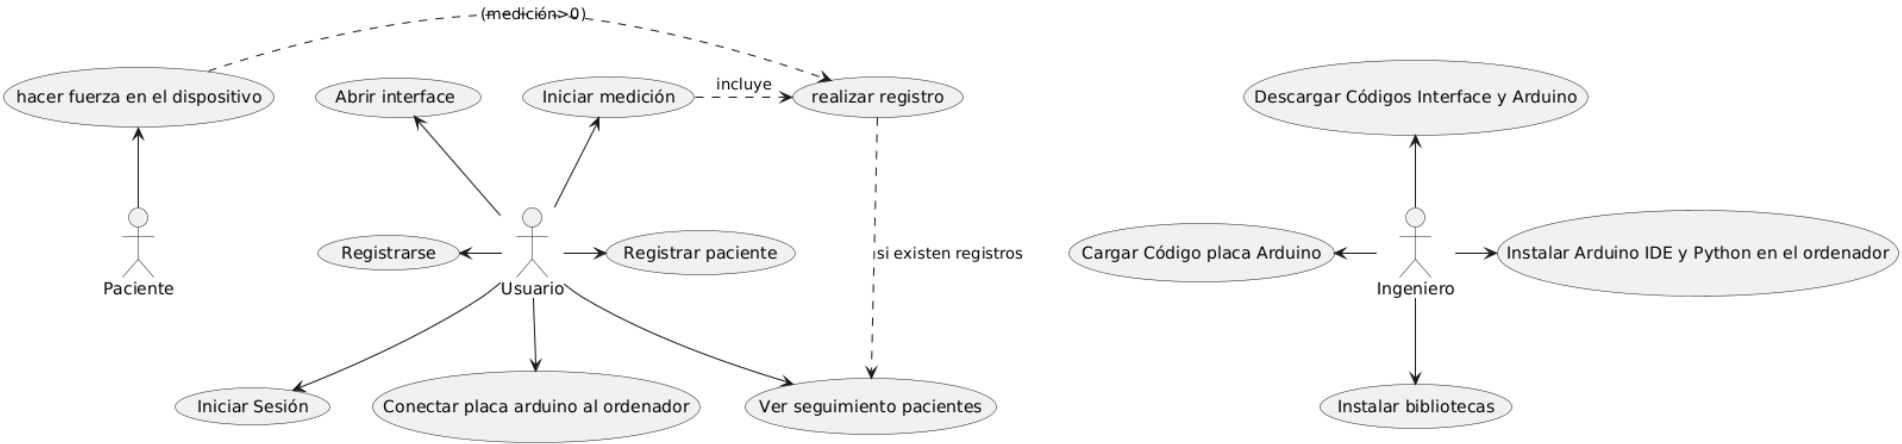
\includegraphics[width=1.15\linewidth]{img/Diagrama Casos de Uso.png}
    \caption{Diagrama Casos de uso. Fuente propia}
    \label{fig:Diagrama Casos de uso}
\end{figure}
\section{Explicación casos de uso.}

En esta sección se van a explicar de forma detallada cada uno de los casos de uso que se realizan, desde la puesta en marcha del dispositivo por los ingenieros hasta su uso en el hospital por los sanitarios.

\begin{table}[p]
	\centering
	\begin{tabularx}{\linewidth}{ p{0.21\columnwidth} p{0.71\columnwidth} }
		\toprule
		\textbf{CU-1}    & \textbf{Instalar Arduino IDE y Python}\\
		\toprule
		\textbf{Versión}        & 1.0    \\
		\textbf{Autor}  & Claudia Valentín Alguacil \\
		\textbf{Descripción}          & Instalación de ambas aplicaciones en el ordenador. \\
		\textbf{Precondición}         & Tener acceso al ordenador del profesional. \\
		\textbf{Acciones}             &
		\begin{enumerate}
			\def\labelenumi{\arabic{enumi}.}
			\tightlist
			\item Acceder a la web de ambas aplicaciones.
			\item Descargarlas en el ordenador.
                \item Instalarlas en el ordenador.
		\end{enumerate}\\
		\textbf{Postcondición}        &  Se podrán abrir ambas aplicaciones y ver el código. \\
		\textbf{Excepciones}          & Sin acceso a internet no se pueden descargar. \\
		\textbf{Importancia}          & Alta \\
		\bottomrule
	\end{tabularx}
	\caption{CU-1 Nombre del caso de uso.}
\end{table}

\begin{table}[p]
	\centering
	\begin{tabularx}{\linewidth}{ p{0.21\columnwidth} p{0.71\columnwidth} }
		\toprule
		\textbf{CU-2}    & \textbf{Cargar código en la placa Arduino }\\
		\toprule
		\textbf{Versión}              & 1.0    \\
		\textbf{Autor}                & Claudia Valentín Alguacil \\
		
		\textbf{Descripción}          & Cargar código que produce que los sensores midan la fuerza generada por el paciente.  \\
		\textbf{Precondición}         & Tener descargado e instalado Arduino IDE. \\
		\textbf{Acciones}             &
		\begin{enumerate}
			\def\labelenumi{\arabic{enumi}.}
			\tightlist
			\item Abrir código Arduino.ino en Arduino IDE.
			\item Conectar placa arduino al ordenador mediante el cable USB.
                \item Mandar el código desde la aplicación a la placa Arduino.
		\end{enumerate}\\
		\textbf{Postcondición}        &  Se puede medir pesos. \\
		\textbf{Excepciones}          & Conectar mal la placa o cable USB roto. \\
		\textbf{Importancia}          & Alta \\
		\bottomrule
	\end{tabularx}
	\caption{CU-2 Cargar código en la placa Arduino.}
\end{table}

\begin{table}[p]
	\centering
	\begin{tabularx}{\linewidth}{ p{0.21\columnwidth} p{0.71\columnwidth} }
		\toprule
		\textbf{CU-3}    & \textbf{Descargar códigos arduino e interfaz}\\
		\toprule
		\textbf{Versión}              & 1.0    \\
		\textbf{Autor}                & Claudia Valentín Alguacil \\
		
		\textbf{Descripción}          & Descargar los códigos que permiten utilizar el dispositivo y la interfaz. \\
		\textbf{Precondición}         & Tener acceso a los códigos. \\
		\textbf{Acciones}             &
		\begin{enumerate}
			\def\labelenumi{\arabic{enumi}.}
			\tightlist
			\item Acceder a la carpeta que contienen los archivos.
			\item Descargarlas en el ordenador.
		\end{enumerate}\\
		\textbf{Postcondición}        &  -- \\
		\textbf{Excepciones}          & Sin acceso a internet no se pueden descargar. \\
		\textbf{Importancia}          & Alta \\
		\bottomrule
	\end{tabularx}
	\caption{CU-3 Descargar los códigos que permiten utilizar el dispositivo y la interfaz}
\end{table}
% Caso de Uso 1 -> Consultar Experimentos.
\begin{table}[p]
	\centering
	\begin{tabularx}{\linewidth}{ p{0.21\columnwidth} p{0.71\columnwidth} }
		\toprule
		\textbf{CU-4} & \textbf{Instalar bibliotecas}\\
		\toprule
		\textbf{Versión}              & 1.0    \\
		\textbf{Autor}                & Claudia Valentín Alguacil \\
		
		\textbf{Descripción}          & Instalación de las bibliotecas necesarias para que el ordenador pueda procesar y abrir la interfaz sin problemas. \\
		\textbf{Precondición}         & Tener descargado python en el ordenador. \\
		\textbf{Acciones}             &
		\begin{enumerate}
			\def\labelenumi{\arabic{enumi}.}
			\tightlist
			\item Acceder al CMD del ordenador.
			\item Instalar una a una las bibliotecas.
		\end{enumerate}\\
		\textbf{Postcondición}        &  Se podrán abrir la interfaz sin ningún problema. \\
		\textbf{Excepciones}          & Si no se instalan correctamente, no se podrá abrir la interfaz. \\
		\textbf{Importancia}          & Alta \\
		\bottomrule
	\end{tabularx}
	\caption{CU-4 Instalar bibliotecas.}
\end{table}

\begin{table}[p]
	\centering
	\begin{tabularx}{\linewidth}{ p{0.21\columnwidth} p{0.71\columnwidth} }
		\toprule
		\textbf{CU-5}    & \textbf{Abrir interfaz}\\
		\toprule
		\textbf{Versión}              & 1.0    \\
		\textbf{Autor}                & Claudia Valentín Alguacil \\
		
		\textbf{Descripción}          & Proceso de abrir la interfaz por parte del sanitario. \\
		\textbf{Precondición}         & Que el ingeniero haya realizado correctamente sus funciones de descarga e instalación de los diferentes paquetes y aplicaciones requeridas. \\
		\textbf{Acciones}             &
        Opción 1: 
		\begin{enumerate}
			\def\labelenumi{\arabic{enumi}.}
			\tightlist
			\item Abrir el CMD del ordenador.
			\item Navegar hasta la carpeta en la que está el código descargado.
                \item Ejecutar el comando:
                
                \$ python app.py
		\end{enumerate}
        Opción dos:
        \begin{itemize}
        \def\labelenumi{\arabic{enumi}.}
		  \tightlist
            \item Abrir Visual Studio Code
            \item Abrir la carpeta donde se encuentra el código descargado.
            \item Ejecutar el comando:
                
            \$ python app.py
        \end{itemize} \\
		\textbf{Postcondición}        &  Se abre la interfaz. \\
		\textbf{Excepciones}          & Que haya algún fallo durante el proceso que realiza el ingeniero o que se acceda mal a la carpeta lo que produciría un error y no se desplegará la interfaz. \\
		\textbf{Importancia}          & Media. \\
		\bottomrule
	\end{tabularx}
	\caption{CU-6 Abrir interfaz.}
\end{table}

\begin{table}[p]
	\centering
	\begin{tabularx}{\linewidth}{ p{0.21\columnwidth} p{0.71\columnwidth} }
		\toprule
		\textbf{CU-7}    & \textbf{Registrarse}\\
		\toprule
		\textbf{Versión}              & 1.0    \\
		\textbf{Autor}                & Claudia Valentín Alguacil \\
		 
		\textbf{Descripción}          & El sanitario se crea una cuenta en la interfaz para que pueda acceder en otras ocasiones. Este proceso produce una recopilación de datos personales como son el nombre, apellidos, nombre de usuario y una contraseña. \\
		\textbf{Precondición}         & Que la interfaz abra correctamente y no tener un usuario ya registrado. \\
		\textbf{Acciones}             &
		\begin{enumerate}
			\def\labelenumi{\arabic{enumi}.}
			\tightlist
			\item Abrir interfaz.
			\item Seleccionar botón de 'Registrarse'.
                \item Rellenar todos los datos requeridos.
                \item Seleccionar botón de 'Registrarse'.
		\end{enumerate}\\
		\textbf{Postcondición}        &  Usuario registrado lo que permitiría acceder a la siguiente pantalla iniciando sesión. \\
		\textbf{Excepciones}          & Realizar mal el proceso de registro. \\
		\textbf{Importancia}          & Media \\
		\bottomrule
	\end{tabularx}
	\caption{CU-7 Nombre del caso de uso.}
\end{table}

\begin{table}[p]
	\centering
	\begin{tabularx}{\linewidth}{ p{0.21\columnwidth} p{0.71\columnwidth} }
		\toprule
		\textbf{CU-8}    & \textbf{Iniciar sesión}\\
		\toprule
		\textbf{Versión}              & 1.0    \\
		\textbf{Autor}                & Claudia Valentín Alguacil \\
		 
		\textbf{Descripción}          & El sanitario inicia sesión en la interfaz lo que permite que pueda visualizar los registros de sus pacientes, registrar nuevas cuantificaciones o pacientes. \\
		\textbf{Precondición}         & Tener una cuenta creada mediante el registro de nuevo usuario. \\
		\textbf{Acciones}             &
		\begin{enumerate}
			\def\labelenumi{\arabic{enumi}.}
			\tightlist
                \item Abrir interfaz.
			\item Seleccionar botón de 'Iniciar sesión'.
                \item Rellenar la información de inicio de  sesión (usuario y contraseña).
                \item Seleccionar botón de 'Iniciar sesión'.
			\item La interfaz verifica la información recibida.
                \item Se accede a otra pantalla donde se puede visualizar los registros de sus pacientes,registrar nuevas cuantificaciones o pacientes.
		\end{enumerate}\\
		\textbf{Postcondición}    &  Acceder a la siguiente pantalla de la interfaz.\\
		\textbf{Excepciones}  & Poner mal el usuario o contraseña. \\
		\textbf{Importancia} & Alta \\
		\bottomrule
	\end{tabularx}
	\caption{CU-8 Iniciar sesión .}
\end{table}

\begin{table}[p]
	\centering
	\begin{tabularx}{\linewidth}{ p{0.21\columnwidth} p{0.71\columnwidth} }
		\toprule
		\textbf{CU-9}    & \textbf{Registrar paciente.}\\
		\toprule
		\textbf{Versión}              & 1.0    \\
		\textbf{Autor}                & Claudia Valentín Alguacil \\
		 
		\textbf{Descripción}          & Registrar el paciente en la interfaz, supone una recolección de datos como su nombre y apellidos que se recogerán en una base de datos. \\
		\textbf{Precondición}  & Que no esté el paciente ya registrado y que el sanitario haya iniciado sesión.\\
		\textbf{Acciones}             &
		\begin{enumerate}
			\def\labelenumi{\arabic{enumi}.}
			\tightlist
                \item Seleccionar botón de 'Registrar paciente'.
                \item Rellenar la información de registro del paciente (nombre y apellidos).
                \item Seleccionar botón de 'Registrar paciente'.
		\end{enumerate}\\
		\textbf{Postcondición} &  Se podrán registrar datos del usuario. \\
		\textbf{Excepciones} & -- \\
		\textbf{Importancia}          & Alta \\
		\bottomrule
	\end{tabularx}
	\caption{CU-9 Registrar paciente.}
\end{table}



\begin{table}[p]
	\centering
	\begin{tabularx}{\linewidth}{ p{0.21\columnwidth} p{0.71\columnwidth} }
		\toprule
		\textbf{CU-10}    & \textbf{Conectar la placa de arduino al ordenador.}\\
		\toprule
		\textbf{Versión}              & 1.0    \\
		\textbf{Autor}                & Claudia Valentín Alguacil \\
		 
		\textbf{Descripción}          & Conectar el cable USB de la placa de arduino al puerto USB del ordenador. \\
		\textbf{Precondición} & Tener el dispositivo (placa de arduino y sensores).\\
		\textbf{Acciones}             &
		\begin{enumerate}
			\def\labelenumi{\arabic{enumi}.}
			\tightlist
			\item Conectar cable USB al puerto USB del ordenador.
		\end{enumerate}\\
		\textbf{Postcondición}        &  Se podrá realizar la cuantificación de la presión ejercida. \\
		\textbf{Excepciones}          & Conectar mal el USB. \\
		\textbf{Importancia}          & Alta. \\
		\bottomrule
	\end{tabularx}
	\caption{CU-10 Conectar la placa de arduino al ordenador.}
\end{table}

\begin{table}[p]
	\centering
	\begin{tabularx}{\linewidth}{ p{0.21\columnwidth} p{0.71\columnwidth} }
		\toprule
		\textbf{CU-11}    & \textbf{Iniciar medición}\\
		\toprule
		\textbf{Versión}              & 1.0    \\
		\textbf{Autor}                & Claudia Valentín Alguacil \\
		 
		\textbf{Descripción}          & Proceso de cuantificar los valores que recoge los sensores. \\
		\textbf{Precondición}         & Conectar placa de arduino al ordenador y tener desplegada la interfaz. \\
		\textbf{Acciones}             &
		\begin{enumerate}
			\def\labelenumi{\arabic{enumi}.}
			\tightlist
			\item Seleccionar al paciente con el que se quiera registrar una nueva cuantificación.
			\item Conectar la placa de arduino al ordenador.
                \item Seleccionar botón iniciar medición de la interfaz y pulsar el pin botón del dispositivo.
		\end{enumerate}\\
		\textbf{Postcondición}        &  Luz led se enciende.\\
		\textbf{Excepciones}          & No conectar la placa al ordenador. \\
		\textbf{Importancia}          & Media \\
		\bottomrule
	\end{tabularx}
	\caption{CU-11 Iniciar medición.}
\end{table}

\begin{table}[p]
	\centering
	\begin{tabularx}{\linewidth}{ p{0.21\columnwidth} p{0.71\columnwidth} }
		\toprule
		\textbf{CU-12}    & \textbf{Ejercer fuerza en los sensores}\\
		\toprule
		\textbf{Versión}              & 1.0    \\
		\textbf{Autor}                & Claudia Valentín Alguacil \\
		 
		\textbf{Descripción}          & El paciente debe de realizar fuerza en los sensores del dispositivo, colocando cada dedo según el sensor en el que corresponde. \\
		\textbf{Precondición}         &  Casos de Uso: 09, 11 y 12\\
		\textbf{Acciones}             &
		\begin{enumerate}
			\def\labelenumi{\arabic{enumi}.}
			\tightlist
			\item Conectar placa arduino al ordenador.
			\item Seleccionar iniciar medición.
                \item Hacer fuerza en la mano.
		\end{enumerate}\\
		\textbf{Postcondición}        &  Se podrá observar los datos recogidos en la tabla. \\
		\textbf{Excepciones}          & Mala captación de datos. \\
		\textbf{Importancia}          & Media. \\
		\bottomrule
	\end{tabularx}
	\caption{CU-12 Hacer fuerza en el dispositivo.}
\end{table}

\begin{table}[p]
	\centering
	\begin{tabularx}{\linewidth}{ p{0.21\columnwidth} p{0.71\columnwidth} }
		\toprule
		\textbf{CU-13}    & \textbf{Ver seguimiento pacientes}\\
		\toprule
		\textbf{Versión}              & 1.0    \\
		\textbf{Autor}                & Claudia Valentín Alguacil \\
		
		\textbf{Descripción}          & Visualización de los registros de los pacientes realizados mediante la cuantificación de la presión/fuerza que se ejerce a los sensores.\\
		\textbf{Precondición}         & Tener registros \\
		\textbf{Acciones}             &
		\begin{enumerate}
			\def\labelenumi{\arabic{enumi}.}
			\tightlist
			\item Acceder a la pantalla del paciente del que queramos observar el seguimiento.
			\item Seleccionar 'Visualización Registro'.
                \item Visualizar todos los registros realizados.
		\end{enumerate}\\
		\textbf{Postcondición}        &  -- \\
		\textbf{Excepciones}          & -- \\
		\textbf{Importancia}          & Baja/Media \\
		\bottomrule
	\end{tabularx}
	\caption{CU-13 Ver seguimiento pacientes.}
\end{table}


\newpage

\section{Prototipos de interfaz o interacción con el proyecto.}

Para este proyecto se ha diseñado un prototipo de interfaz para ordenador tipo desplegable, en base a las necesidades y requisitos para su uso. 

Esta interfaz creada consta de 8 pantallas:
\begin{enumerate}
    \item Pantalla Principal: es la pantalla de presentación (véase \textit{Figura} \ref{fig:Pantalla principal}), en ella se muestra el logo de la aplicación, dos botones, iniciar sesión y registrarse, y un recuadro con información relevante sobre la interfaz.
    \begin{figure}
        \centering
        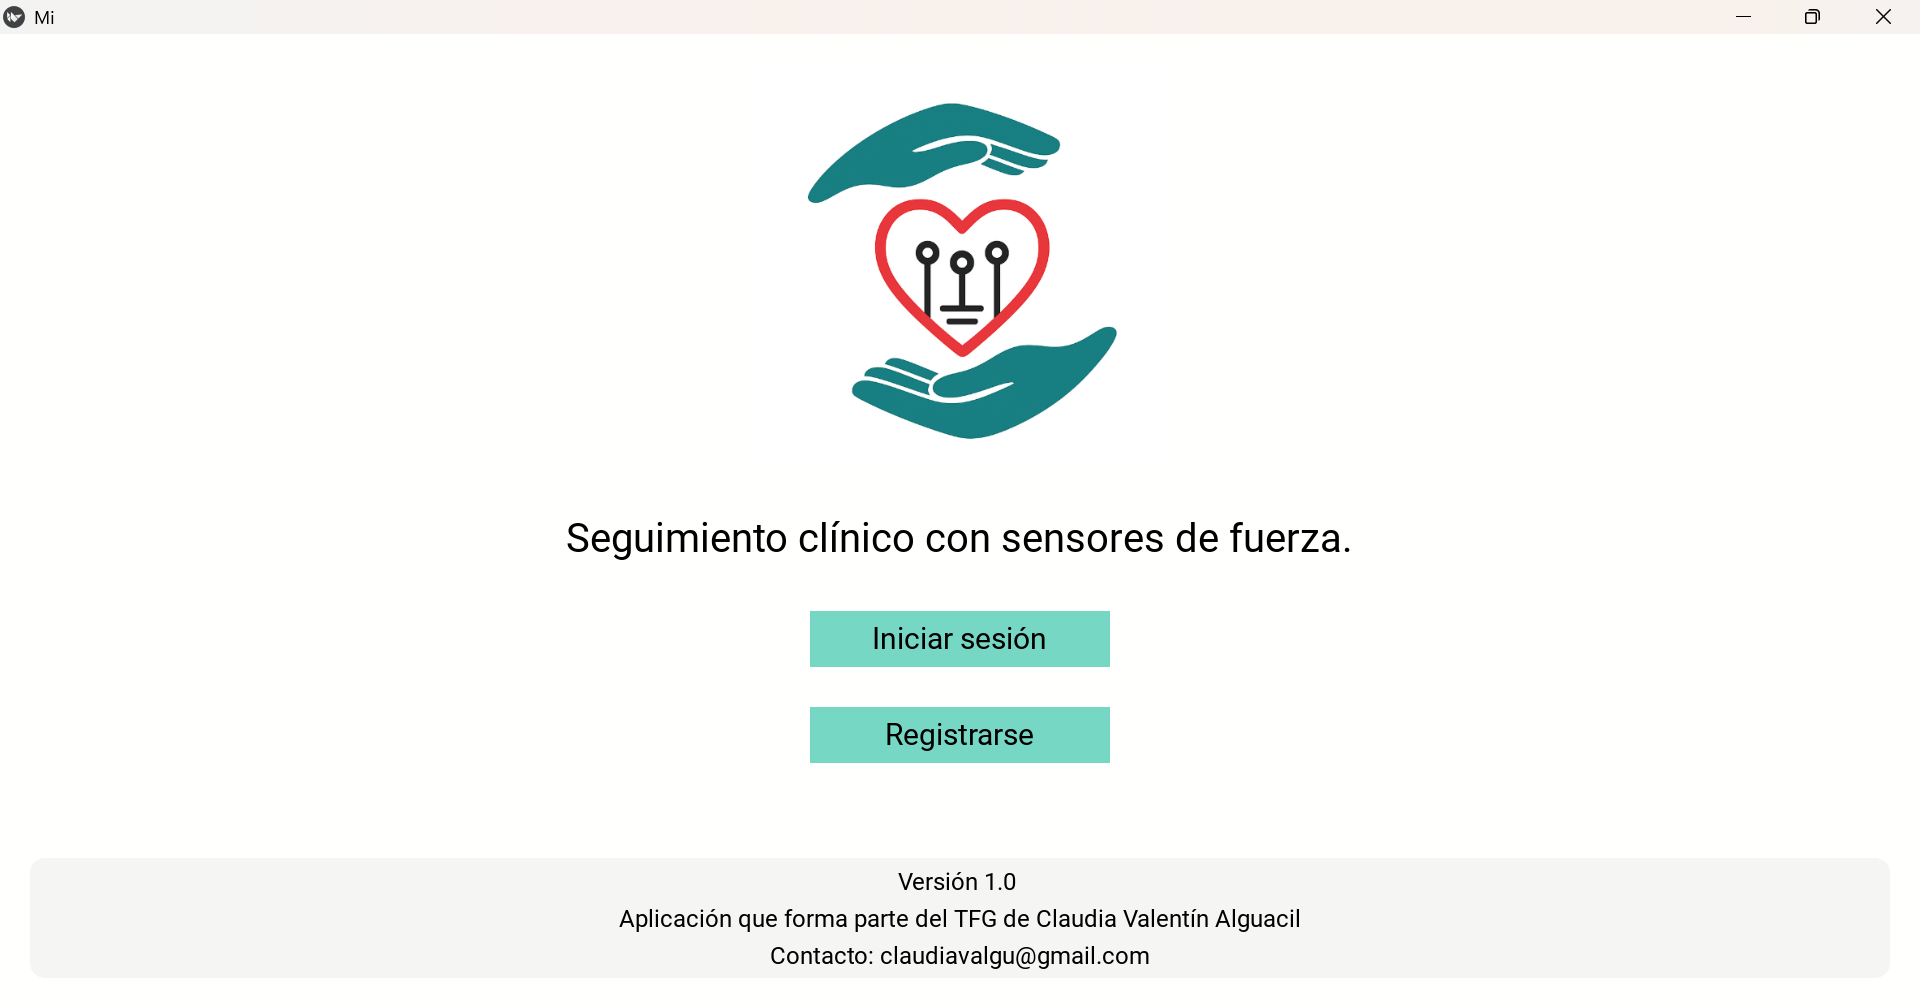
\includegraphics[width=1\linewidth]{img/Pantalla principal.png}
        \caption{Pantalla principal. Fuente Propia.}
        \label{fig:Pantalla principal}
    \end{figure}
    \item Pantalla Inicio Sesión: es la pantalla que permite al usuario (sanitario) iniciar sesión en la interfaz (véase \textit{Figura} \ref{fig:Pantalla Inicio Sesión}), en ella se debe introducir el usuario y contraseña personal de cada usuario para acceder al área. Desde esta pantalla, se puede volver a la pantalla principal seleccionando el botón 'Volver' o bien, acceder a la siguiente pantalla seleccionando el botón 'Entrar'.
\begin{figure}
    \centering
    \includegraphics[width=1\linewidth]{img/Pantalla Inicio Sesión.png}
    \caption{Pantalla Inicio Sesión. Fuente Propia.}
    \label{fig:Pantalla Inicio Sesión}
\end{figure}
    \item Pantalla Registrar Usuario: es la pantalla que permite al usuario (sanitario) registrarse en la interfaz (véase \textit{Figura} \ref{fig:Pantalla Registrar Usuario}), en ella se debe introducir el nombre, apellidos, nombre de usuario y contraseña personal. Estos datos se almacenarán en un documento Json. Desde esta pantalla, se puede volver a la pantalla principal sin registrar un nuevo usuario seleccionando el botón 'Volver' o bien, registrar un nuevo usuario seleccionando el botón 'Registrarse'. Realizando la última acción la aplicación te dirige de forma automático a la pantalla principal.
    \begin{figure}
        \centering
        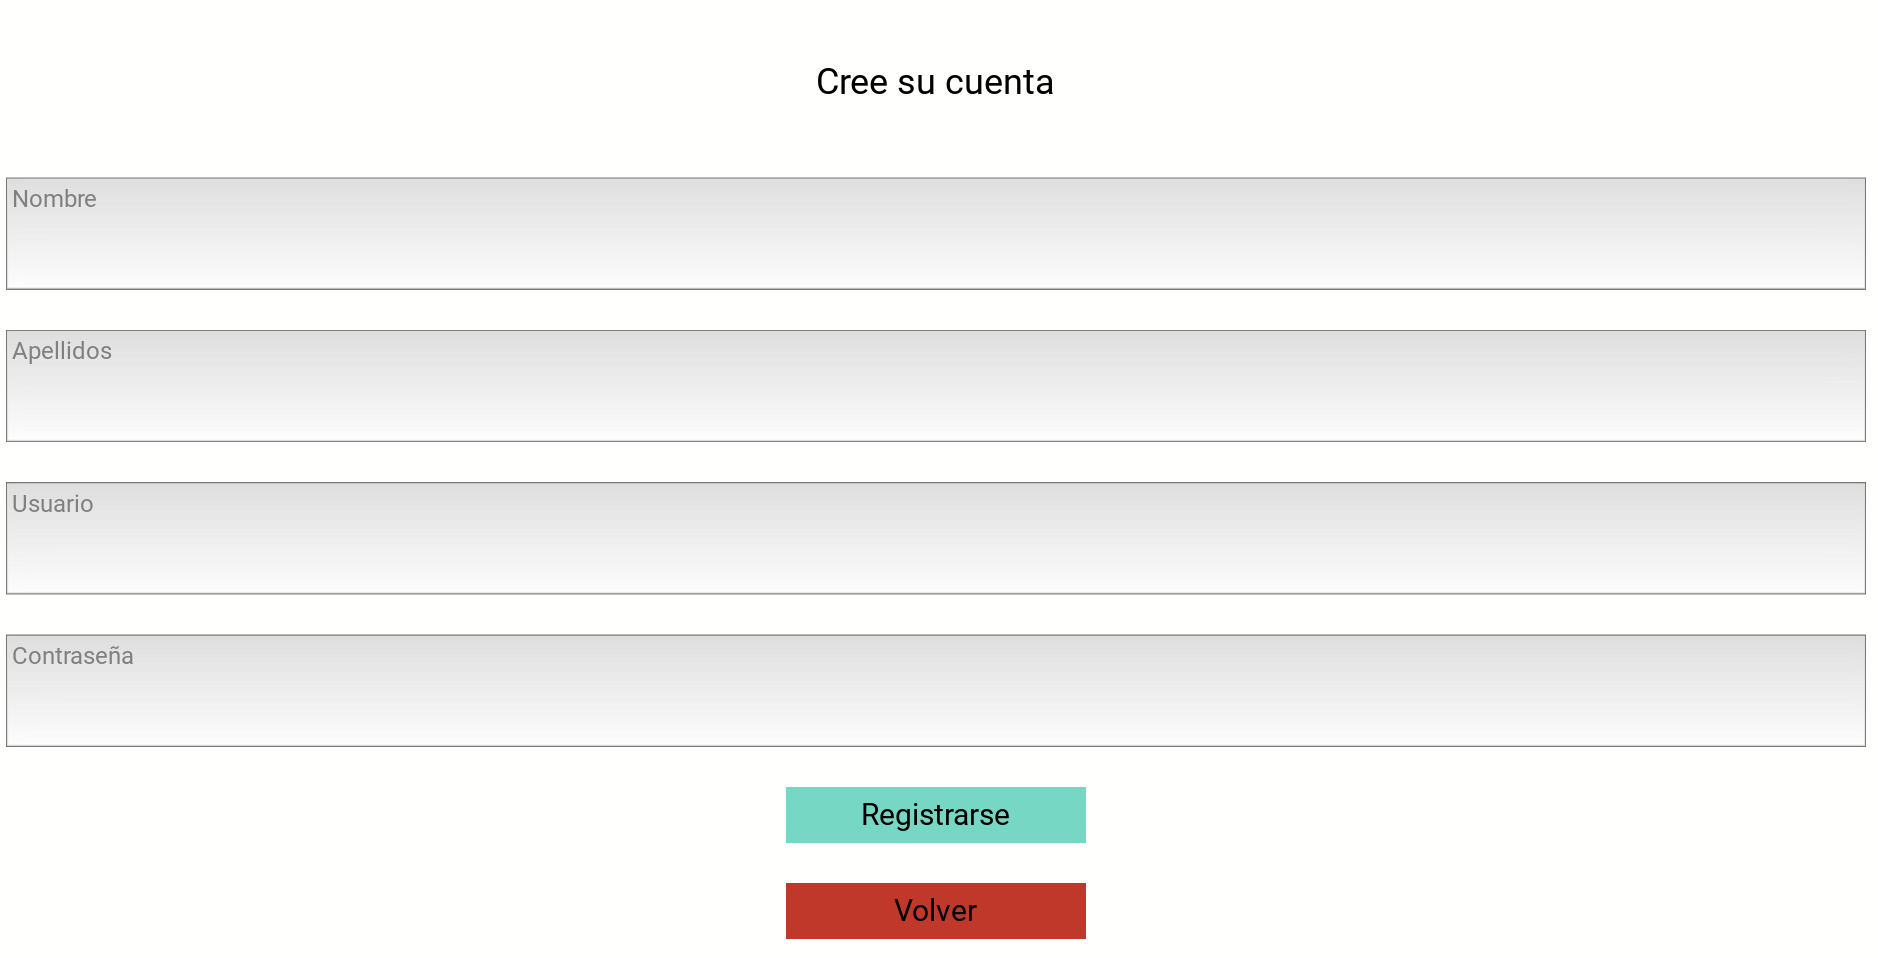
\includegraphics[width=1\linewidth]{img/Pantalla Registrar Usuario.png}
        \caption{Pantalla Registrar Usuario. Fuente propia}
        \label{fig:Pantalla Registrar Usuario}
    \end{figure}
    \item Pantalla de Inicio: es la pantalla principal de cada usuario (véase \textit{Figura} \ref{fig:Pantalla Inicio}). Consta de un recuadro con el nombre y apellidos del profesional, un mensaje de bienvenida y dos botones, uno de seleccionar paciente y otro de registrar paciente. Si seleccionamos el primero de ellos, sale un menú desplegable con los diferentes nombres y apellidos de los pacientes registrados. Si seleccionamos el segundo botón, nos dirige a una pantalla nueva que nos permitirá el registro de un nuevo paciente.
    \begin{figure}
        \centering
        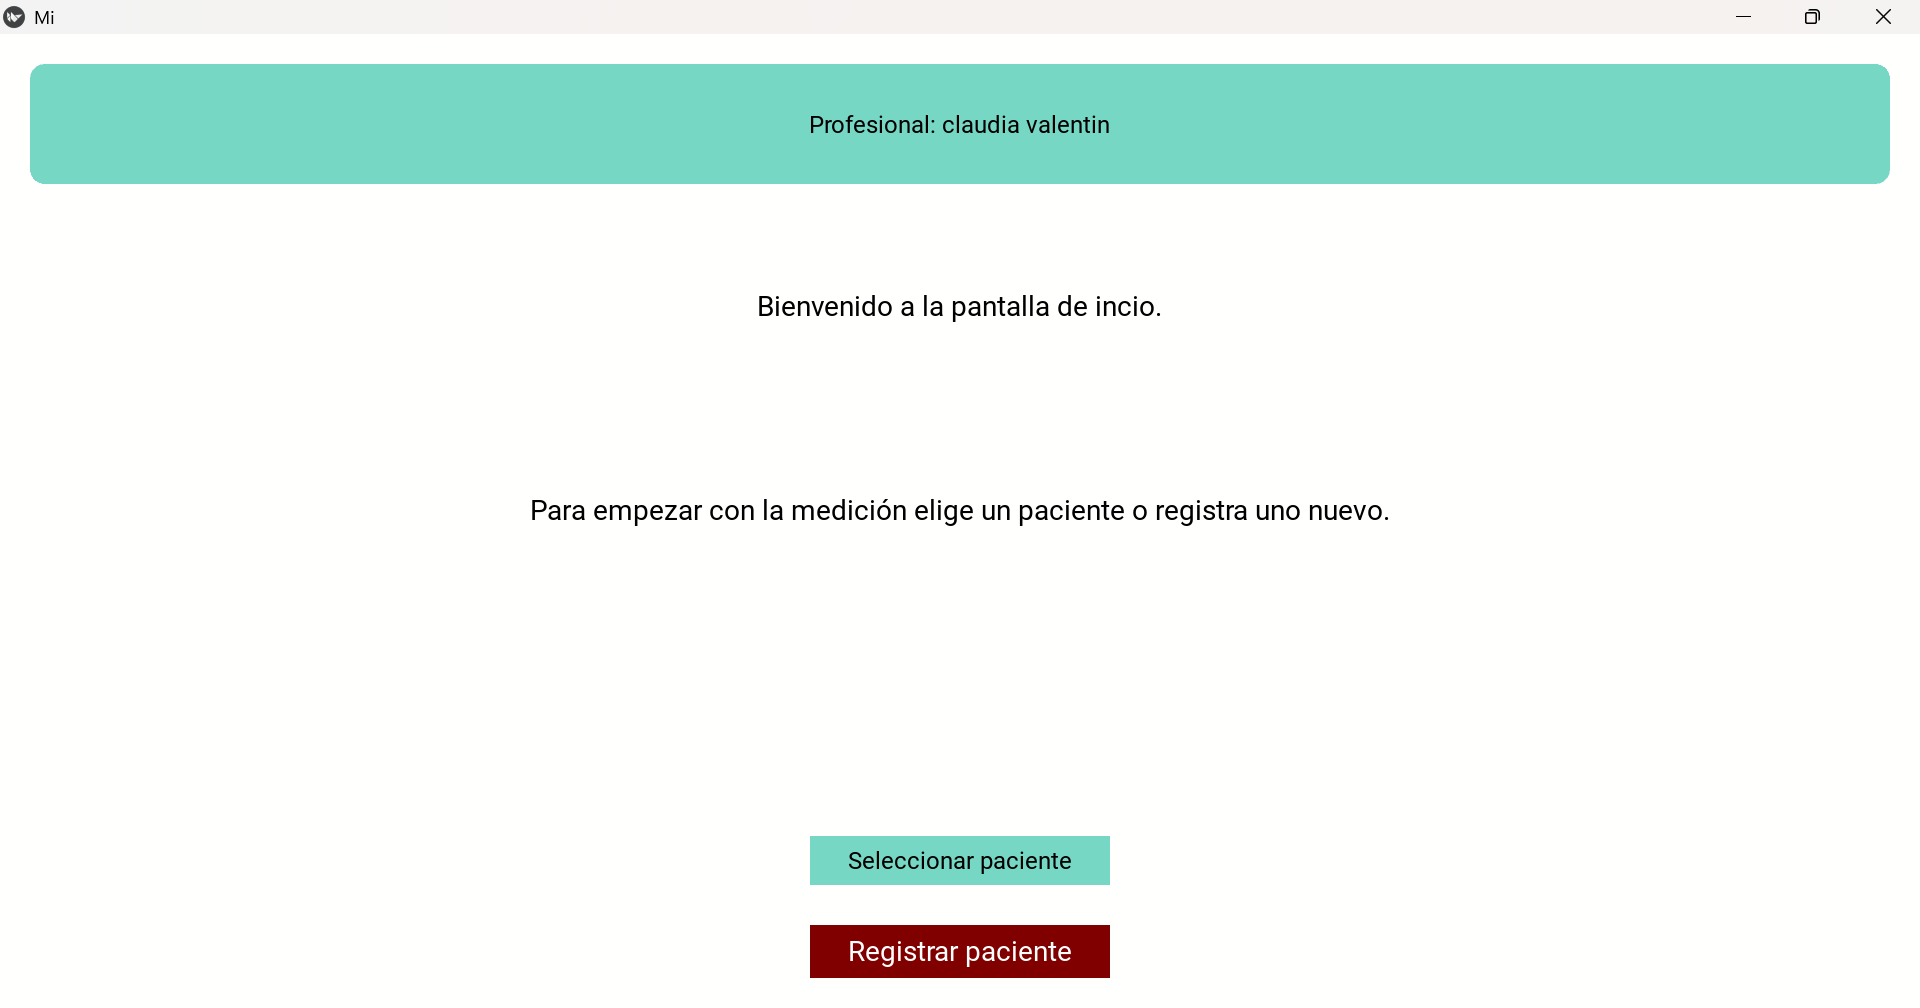
\includegraphics[width=1\linewidth]{img/Pantalla Inicio.png}
        \caption{Pantalla Inicio. Fuente Propia}
        \label{fig:Pantalla Inicio}
    \end{figure}
    \item Pantalla Registrar paciente: es la pantalla que permite al usuario (sanitario) registrar a un nuevo paciente en la base de datos (véase \textit{Figura} \ref{fig:Pantalla registrar Paciente}), en ella se debe introducir el nombre y apellidos del paciente. Estos datos se almacenarán en un documento Excel, donde, además, se guardarán las diferentes cuantificaciones de fuerza. Desde esta pantalla, se puede volver a la pantalla principal sin registrar un nuevo paciente seleccionando el botón 'Volver' o bien, registrar un nuevo paciente seleccionando el botón 'Registrar paciente'. Realizando la última acción la aplicación te dirige de forma automática a la pantalla de inicio.
    \begin{figure}
        \centering
        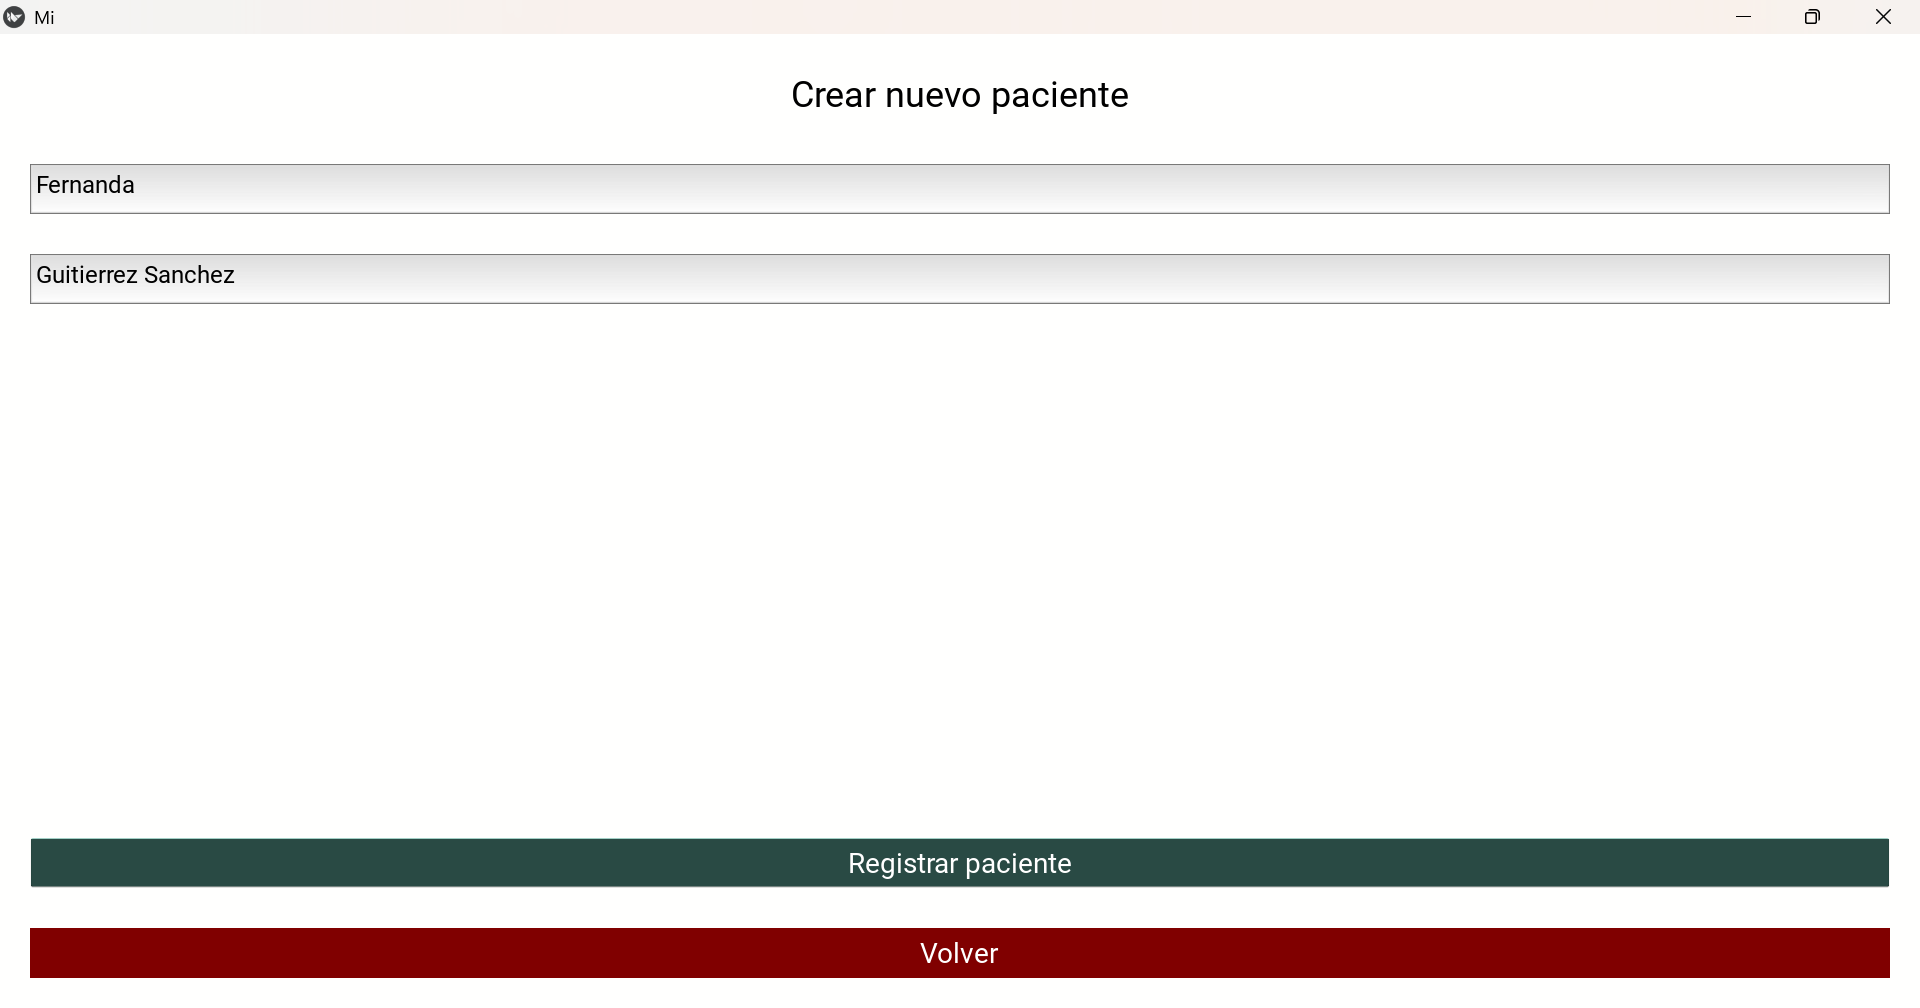
\includegraphics[width=1\linewidth]{img/Pantalla registrar Paciente.png}
        \caption{Pantalla registrar Paciente. Fuente propia}
        \label{fig:Pantalla registrar Paciente}
    \end{figure}
    \item Pantalla paciente: es la pantalla general de cada paciente (véase \textit{Figura} \ref{fig:Pantalla paciente}). Esta contiene un recuadro superior con el nombre y apellidos del paciente y 4 botones, 'Iniciar medición', 'Visualización registro', 'Visualización gráfica' y 'Volver. Al pulsar sobre el primero de ellos realiza el proceso de medir la fuerza ejercida en los sensores, esta cuantificación se guarda automáticamente en una base de datos. Al pulsar sobre el segundo y tercer botón se abre una pantalla nueva, y al pulsar sobre el último botón vuelve a la pantalla de inicio.
    \begin{figure}
        \centering
        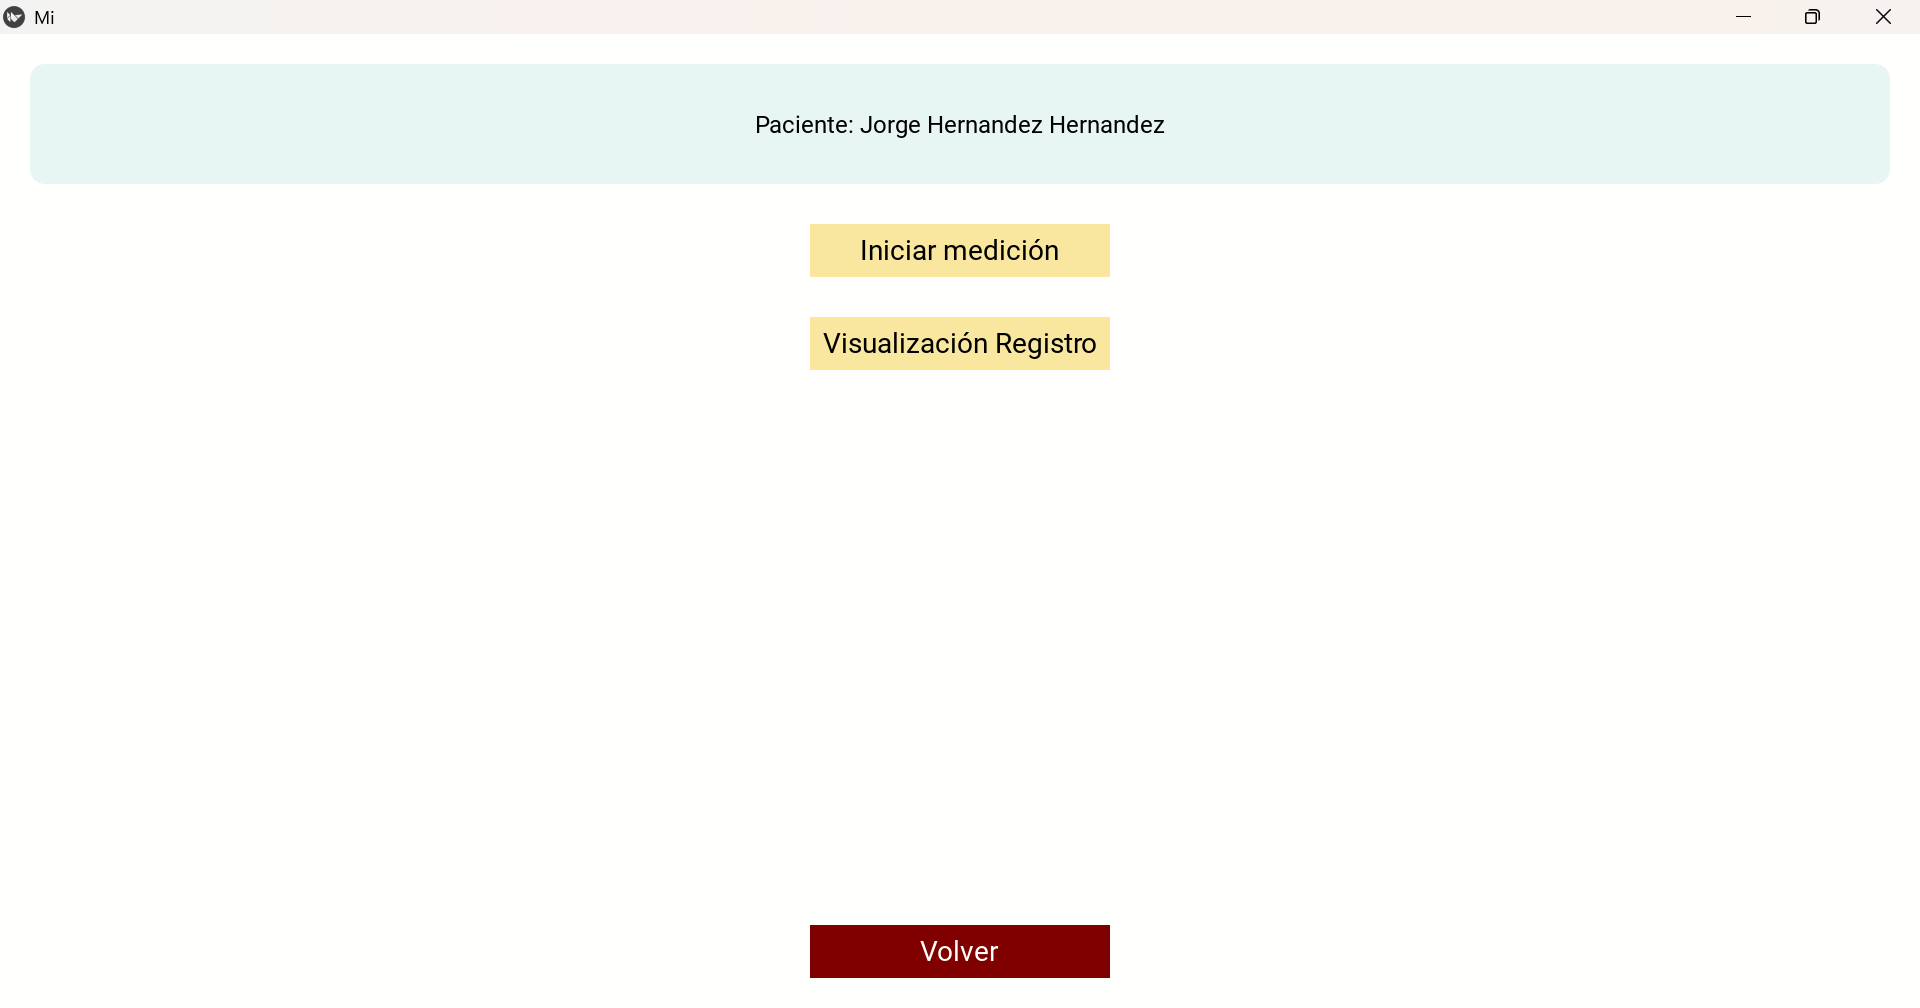
\includegraphics[width=1\linewidth]{img/Pantalla paciente.png}
        \caption{Pantalla paciente. Fuente propia}
        \label{fig:Pantalla paciente}
    \end{figure}
    \item Pantalla visualización: es la pantalla a la que se accede al pulsar el botón 'Visualización registro' en la pantalla paciente. En ella se muestra el registro de las mediciones realizadas por el paciente (véase \textit{Figura} \ref{fig:Pantalla visualización}). Tiene un botón 'Volver' para poder volver a la pantalla paciente y hacer nuevas mediciones, ver los registros en formato gráfica o seguir volviendo atrás y elegir un paciente nuevo.
    \begin{figure}
        \centering
        \includegraphics[width=1\linewidth]{img/Pantalla visualización.png}
        \caption{Pantalla visualización registros. Fuente propia}
        \label{fig:Pantalla visualización}
    \end{figure}
    \item Pantalla visualización gráfica: es la pantalla a la que se accede al pulsar el botón 'Visualización gráfica' en la pantalla paciente. En ella se muestra el registro de las mediciones realizadas por el paciente en forma de una gráfica de líneas. (véase \textit{Figura} \ref{fig:Pantalla grafica}). Tiene un botón 'Volver' para poder volver a la pantalla paciente y hacer nuevas mediciones, ver los registros en formato tabla o seguir volviendo atrás y elegir un paciente nuevo.
    \begin{figure}
        \centering
        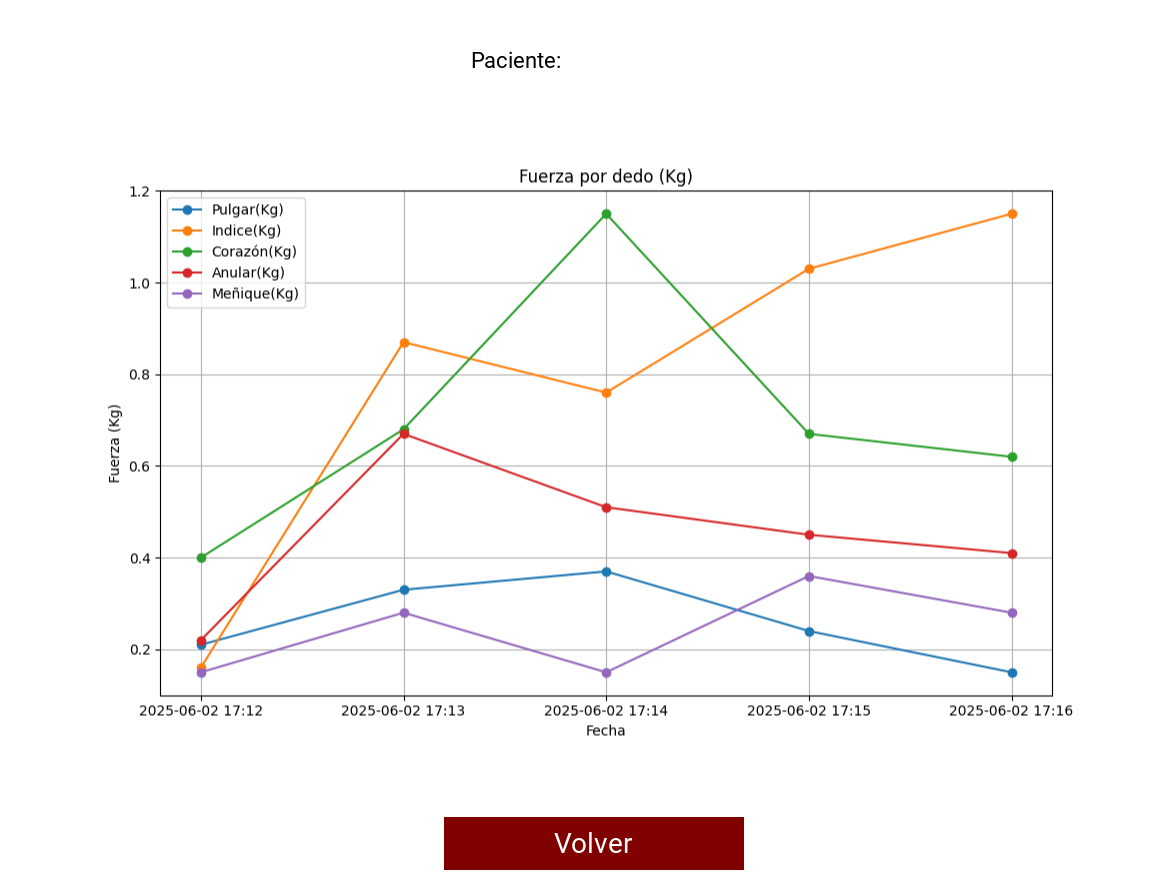
\includegraphics[width=0.75\linewidth]{img/Pantalla grafica.png}
        \caption{Pantalla visualización registros formato gráfica. Fuente propia}
        \label{fig:Pantalla grafica}
    \end{figure}
\end{enumerate}